\subsection{Générateur d'instances}

Pour générer une instance de \textit{Palisade}, il n'est pas raisonnable de placer les indices au hasard. En pratique, cette approche produit très souvent des grilles incohérentes, ou tout simplement sans solution. Nous avons donc choisi de construire le puzzle à l'envers : on commence par créer une grille déjà résolue, c'est-à-dire une partition correcte en régions connexes, puis on en déduit ensuite les murs et les indices.

Cette construction impose aussi une contrainte simple sur les dimensions. Si la grille contient \(n \times m\) cases et que l'on veut la découper en \(k\) régions, alors le nombre total de cases doit être divisible par \(k\). Autrement dit, il faut avoir :
\[
k \mid (n \times m).
\]
Quand cette condition est vérifiée, la taille de chaque région est calculée automatiquement par
\[
s = \frac{n \times m}{k}.
\]
Dans la version classique de \textit{Palisade}, on fixe généralement \(s = 5\). Dans notre générateur, ce n'est plus une constante : la valeur de \(s\) dépend directement des dimensions de la grille et du nombre de régions choisi.

La génération elle-même repose sur un parcours en profondeur (\textit{Depth-First Search}, DFS) avec \textit{backtracking}. La grille est d'abord vide, puis les régions sont construites une par une. Pour chaque région, on choisit une case de départ libre, puis on ajoute progressivement des cases voisines. Le choix des voisins est fait de manière aléatoire pour obtenir des instances variées. Si un choix bloque la suite de la construction, l'algorithme revient en arrière et essaie une autre possibilité. Cette méthode permet de garder des régions connexes et d'éviter de laisser des cases isolées qu'il serait ensuite impossible d'intégrer correctement.

Une fois les régions construites, le calcul des indices est direct. Pour chaque case, on regarde ses quatre côtés. Un côté compte dans l'indice s'il correspond au bord extérieur de la grille, ou s'il sépare deux régions différentes. L'indice d'une case est donc simplement le nombre de frontières qui l'entourent. À partir de cette étape, on obtient à la fois la position des murs et les valeurs numériques affichées dans la grille.

Enfin, on ne conserve pas forcément tous les indices. Pour régler la difficulté, on utilise un paramètre probabiliste \texttt{fill\_ratio}. Chaque indice est gardé avec une certaine probabilité, puis masqué sinon. On obtient ainsi une grille partiellement remplie, cohérente avec la solution construite au départ, mais suffisamment incomplète pour former un vrai puzzle.

La Figure~\ref{fig:palisade-generation-flow} résume les grandes étapes du générateur.

\begin{figure}[H]
    \centering
    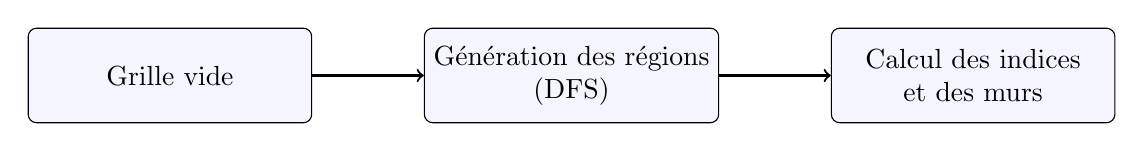
\begin{tikzpicture}[
        every node/.style={
            draw,
            rounded corners=3pt,
            align=center,
            minimum width=3.6cm,
            minimum height=1.2cm,
            fill=blue!4
        }
    ]
        \node (empty) at (0,0) {Grille vide};
        \node (regions) at (5.1,0) {Génération des régions\\(DFS)};
        \node (clues) at (10.2,0) {Calcul des indices\\et des murs};

        \draw[->, thick] (empty) -- (regions);
        \draw[->, thick] (regions) -- (clues);
    \end{tikzpicture}
    \caption{Chaîne conceptuelle du générateur d'instances pour \textit{Palisade}.}
    \label{fig:palisade-generation-flow}
\end{figure}
